\documentclass[11pt,table]{beamer}
\mode<presentation>
\usepackage{etex}
\usepackage{graphicx}
\usepackage{epstopdf}
\usepackage[english]{babel}
\usepackage{tabularx}
\usepackage{booktabs}
\usepackage{mathrsfs}
\usepackage{multicol}
\usepackage{bm}
\usepackage{subcaption}
\usepackage{wrapfig}
\usepackage{dcolumn}
\usepackage{threeparttable}
\usepackage{booktabs}
\usepackage{bbm}
\usepackage{amsmath,dsfont,listings}
\usepackage{amssymb}
\usepackage{rotating}
\usepackage{multirow}
\usepackage{tcolorbox}
\usepackage[authoryear]{natbib}
\usepackage{circledsteps}
\usepackage{qtree}

\usepackage{tikz}
\usetikzlibrary{arrows,decorations.pathmorphing,backgrounds,fit,positioning,shapes.symbols,chains}
\setbeamertemplate{section in toc}[sections numbered]
\setbeamertemplate{caption}[numbered]

\bibliographystyle{Econometrica}

\setbeamersize{text margin right=3.5mm, text margin left=7.5mm}  % text margin
\setbeamersize{sidebar width left=0cm, sidebar width right=0mm}
\setbeamertemplate{sidebar right}{}
\setbeamertemplate{sidebar left}{}

\definecolor{text-grey}{rgb}{0.45, 0.45, 0.45} % grey text on white background
\definecolor{bg-grey}{rgb}{0.66, 0.65, 0.60} % grey background (for white text)
\definecolor{fu-blue}{RGB}{0, 51, 102} % blue text
\definecolor{fu-green}{RGB}{153, 204, 0} % green text
\definecolor{fu-red}{RGB}{204, 0, 0} % red text (used by \alert)
\definecolor{BrewerBlue}{HTML}{377EB8} % Define Brewer Blue
\definecolor{BrewerRed}{HTML}{E41A1C}  % Define Brewer Red

\setbeamertemplate{frametitle}{%
    \vskip-30pt \color{text-grey}\large%
    \begin{minipage}[b][23pt]{\textwidth}%
    \flushleft\insertframetitle%
    \end{minipage}%
}

\setbeamertemplate{navigation symbols}{} 

%%% begin title page
\setbeamertemplate{title page}{
\vskip2pt\hfill
\vskip19pt\hskip3pt

% set the title and the author
\vskip4pt
\parbox[top][1.35cm][c]{11cm}{\LARGE\color{text-grey} \textcolor{red1}{RL}earning:\\[1ex] \inserttitle \\[1ex] \small \quad \\[3ex]}
\vskip17pt
\parbox[top][1.35cm][c]{11cm}{\small Unit 3-4: \insertsubtitle \\[2ex] \insertauthor \\[1ex]}
}
%%% end title page

%%% colors
\usecolortheme{lily}
\setbeamercolor*{normal text}{fg=black,bg=white}
\setbeamercolor*{alerted text}{fg=fu-red}
\setbeamercolor*{example text}{fg=fu-green}
\setbeamercolor*{structure}{fg=fu-blue}

\setbeamercolor*{block title}{fg=white,bg=black!50}
\setbeamercolor*{block title alerted}{fg=white,bg=black!50}
\setbeamercolor*{block title example}{fg=white,bg=black!50}

\setbeamercolor*{block body}{bg=black!10}
\setbeamercolor*{block body alerted}{bg=black!10}
\setbeamercolor*{block body example}{bg=black!10}

\setbeamercolor{bibliography entry author}{fg=fu-blue}
\setbeamercolor{bibliography entry journal}{fg=text-grey}
\setbeamercolor{item}{fg=fu-blue}
\setbeamercolor{navigation symbols}{fg=text-grey,bg=bg-grey}
%%% end colors

%%% headline
\setbeamertemplate{headline}{
\vskip30pt
}
%%% end headline

%%% footline
\newcommand{\footlinetext}{
%\insertshortinstitute, \insertshorttitle, \insertshortdate
}
\setbeamertemplate{footline}{
\vskip2pt
\hfill \raisebox{-1pt}{\usebeamertemplate***{navigation symbols}}
\hfill \insertframenumber\hspace{10pt}
\vskip4pt
}
%%% end footline

%%% settings for listings package
\lstset{extendedchars=true, showstringspaces=false, basicstyle=\footnotesize\sffamily, tabsize=2, breaklines=true, breakindent=10pt, frame=l, columns=fullflexible}
\lstset{language=Java} % this sets the syntax highlighting
\lstset{mathescape=true} % this switches on $...$ substitution in code
% enables UTF-8 in source code:
\lstset{literate={ä}{{\"a}}1 {ö}{{\"o}}1 {ü}{{\"u}}1 {Ä}{{\"A}}1 {Ö}{{\"O}}1 {Ü}{{\"U}}1 {ß}{\ss}1}
%%% end listings

\usepackage{concmath}
\usepackage{xcolor}
\definecolor{red1}{RGB}{206, 17, 38}
\definecolor{blue1}{RGB}{16, 118, 208}
\definecolor{gray1}{RGB}{117, 115, 115}
\usepackage{hyperref}


\newtheorem{proposition}{Proposition}
\newtheorem{assumption}{Definition}

\title[]{Short guides to reinforcement learning}
\subtitle[]{Q-Learning}
\author[D. Rostam-Afschar]{\textcolor{gray1}{Davud Rostam-Afschar (Uni Mannheim)}}
\date[]{\today}
\subject{Econometrics}
\renewcommand{\footlinetext}{\insertshortinstitute, \insertshorttitle, \insertshortdate}
\hypersetup{
    bookmarks=false,
    unicode=false,
    pdftoolbar=false,
    pdffitwindow=true,
    pdftitle={Reinforcement Learning for Business, Economics, and Social Sciences: \insertsubtitle},
    pdfauthor={Davud Rostam-Afschar},
    pdfsubject={Reinforcement Learning},
    pdfkeywords={reinforcement learning, Q-Learning},
    pdfnewwindow=true,
}
\def\sym#1{\ifmmode^{#1}\else\(^{#1}\)\fi}

\begin{document}

\begin{frame}[plain]
  \titlepage
\end{frame}

% --------------------------------------------------- Slide --
%\begin{frame}
	%\frametitle{Content}
	%\tableofcontents[]
%\end{frame}

\section{Q-Learning}
{
\setbeamercolor{background canvas}{bg=BrewerBlue}
\begin{frame}
\centering
\Huge
\textcolor{white}{At this state how much good stuff will happen ... if I do THIS?}
\thispagestyle{empty}
\end{frame}
}


\begin{frame}{Important	Components in Reinforcement Learning}


Reinforcement learning agents may or may not include the following components:
\vspace{3mm}

\begin{itemize}
    \item \textcolor{red1}{\textbf{Model:}} $\mathbb{P}\left(s^{\prime} \mid s, a\right), \mathbb{P}(r \mid s, a)$
\begin{itemize}

\item  Environment dynamics and rewards
\end{itemize}
\item \textcolor{red1}{\textbf{Policy:}} $\pi(s)$

\begin{itemize} 
\item Agent action choices
\end{itemize}
\item \textcolor{red1}{\textbf{Value function:}} $V(s)$

\begin{itemize}
\item  Expected total rewards of the agent's policy 
\end{itemize}
\pause
\item \textcolor{red1}{\textbf{Quality function:}} $Q(s,a)$

\begin{itemize}
\item  Expected total rewards of taking a specific action in a given state and then following a particular policy thereafter
\end{itemize}
\end{itemize}
    
\end{frame}


\begin{frame}{Bellman's Equation}
\begin{itemize}
    \item Optimal state value function $V^{*}(s)$

$$
V^{*}(s)=\max _{a} \mathbb{E}[r \mid s, a]+\gamma \sum_{s^{\prime}} \mathbb{P}\left(s^{\prime} \mid s, a\right) V^{*}\left(s^{\prime}\right)
$$

\item Optimal state-action value function $Q^{*}(s, a)$

$$
\textcolor{red1}{Q^{*}(s, a)=\mathbb{E}[r\mid s,a]+\gamma \sum_{s^{\prime}} \mathbb{P}\left(s^{\prime}\mid s,a\right) \max _{a^{\prime}} Q^{*}\left(s^{\prime}, a^{\prime}\right)}
$$

where $V^{*}(s)=\max _{a} Q^{*}(s, a)$\\
\quad\quad\quad $
\pi^{*}(s)=\underset{a}{\operatorname{argmax}} Q^{*}(s, a)
$ 
\end{itemize}    
\end{frame}



\begin{frame}{Temporal Difference}


\begin{center}

\only<1-2>{
\scalebox{0.8}{
\begin{tikzpicture}[line cap=round,line join=round,x=1pt,y=1pt,yscale=-1,xscale=1]

%Shape: Rectangle [id:dp6447651540962223] 
\draw[line width=2pt]   (200.16,40.44) -- (380.23,40.44) -- (380.23,159.75) -- (200.16,159.75) -- cycle ;
%Straight Lines [id:da6664024825726134] 
\draw[line width=1.5pt]    (260.13,40.44) -- (259.38,160.01) ;
%Straight Lines [id:da787984071032432] 
\draw[line width=1.5pt]    (320.04,40.1) -- (320.38,160.34) ;
%Straight Lines [id:da35411861555941715] 
\draw[line width=1.5pt]    (200.16,99.77) -- (380.23,100.38) ;
%Shape: Square [id:dp6482811179722225] 
\draw  [fill=BrewerBlue  ,fill opacity=1,line width=1.5pt ] (200.42,40.89) -- (259.75,40.89) -- (259.75,100.22) -- (200.42,100.22) -- cycle ;
%Straight Lines [id:da5628793737066431] 
\draw[line width=1.5pt,-latex]    (243.51,59.79) -- (276.78,59.9) ;
%Straight Lines [id:da8088619056184632] 
\draw[line width=1.5pt,latex-]    (243.51,80.12) -- (276.78,80.15) ;
%Straight Lines [id:da023736429487241528] 
\draw[line width=1.5pt,-latex]    (303,70.2) -- (337.78,70.4) ;
%Straight Lines [id:da08303851898715231] 
\draw[line width=1.5pt,-latex]    (290.23,83) -- (290.23,118) ;

% Text Node
\draw (222.8,60) node [anchor=north west][inner sep=0.75pt]  [font=\LARGE] [align=left] {{\Large $\boldsymbol{S_1}$}};
\draw (282,60) node [anchor=north west][inner sep=0.75pt]  [font=\LARGE] [align=left] {{\Large $\boldsymbol{S_2}$}};
\draw (244,48) node [anchor=north west][inner sep=0.75pt]  [font=\LARGE] [align=left] {{\large $\boldsymbol{73}$}};
\draw (244,84) node [anchor=north west][inner sep=0.75pt]  [font=\LARGE] [align=left] {{\large $\boldsymbol{66}$}};
\draw (291,84) node [anchor=north west][inner sep=0.75pt]  [font=\LARGE] [align=left] {{\large $\boldsymbol{81}$}};
\draw (320,57) node [anchor=north west][inner sep=0.75pt]  [font=\LARGE] [align=left] {{\large $\boldsymbol{100}$}};
\end{tikzpicture}
}
}

\only<3>{
\scalebox{0.8}{

\begin{tikzpicture}[line cap=round,line join=round,x=1pt,y=1pt,yscale=-1,xscale=1]

%Shape: Rectangle [id:dp6447651540962223] 

\draw  [fill={BrewerBlue}] (260.87,40.89) -- (320.21,40.89) -- (320.21,100.22) -- (260.87,100.22) -- cycle ;
\draw[line width=2pt]   (200.16,40.44) -- (380.23,40.44) -- (380.23,159.75) -- (200.16,159.75) -- cycle ;
%Straight Lines [id:da6664024825726134] 
\draw[line width=1.5pt]    (260.13,40.44) -- (259.38,160.01) ;
%Straight Lines [id:da787984071032432] 
\draw[line width=1.5pt]    (320.04,40.1) -- (320.38,160.34) ;
%Straight Lines [id:da35411861555941715] 
\draw[line width=1.5pt]    (200.16,99.77) -- (380.23,100.38) ;
%Shape: Square [id:dp6482811179722225] 


%\draw  [fill=bluegray  ,fill opacity=1,line width=1.5pt ] (200.42,40.89) -- (259.75,40.89) -- (259.75,100.22) -- (200.42,100.22) -- cycle ;
%Straight Lines [id:da5628793737066431] 
\draw[line width=1.5pt,-latex]    (243.51,59.79) -- (276.78,59.9) ;
%Straight Lines [id:da8088619056184632] 
\draw[line width=1.5pt,latex-]    (243.51,80.12) -- (276.78,80.15) ;
%Straight Lines [id:da023736429487241528] 
\draw[line width=1.5pt,-latex]    (303,70.2) -- (337.78,70.4) ;
%Straight Lines [id:da08303851898715231] 
\draw[line width=1.5pt,-latex]    (290.23,83) -- (290.23,118) ;

% Text Node
%\draw (222.8,60) node [anchor=north west][inner sep=0.75pt]  [font=\LARGE] [align=left] {{\Large $\boldsymbol{S_1}$}};
\draw (282,60) node [anchor=north west][inner sep=0.75pt]  [font=\LARGE] [align=left] {{\Large $\boldsymbol{S_2}$}};
\draw (244,48) node [anchor=north west][inner sep=0.75pt]  [font=\LARGE] [align=left,color=red] {{\large $\boldsymbol{81.5}$}};
\draw (244,84) node [anchor=north west][inner sep=0.75pt]  [font=\LARGE] [align=left] {{\large $\boldsymbol{66}$}};
\draw (291,84) node [anchor=north west][inner sep=0.75pt]  [font=\LARGE] [align=left] {{\large $\boldsymbol{81}$}};
\draw (320,57) node [anchor=north west][inner sep=0.75pt]  [font=\LARGE] [align=left] {{\large $\boldsymbol{100}$}};
\end{tikzpicture}
}
}

$\gamma=0.9, \alpha=0.5, r=0 \text { for non-terminal states }$

\uncover<2-3>{

\begin{align}
Q(s_{1},right)&=Q(s_{1},right)+\alpha \bigg(r+\gamma \max _{a^{\prime}} Q(s_{2}, a^{\prime})-Q(s_{1},right)\bigg)\nonumber\\
& =73+0.5(0+0.9 \max \{66,81,100\}-73) \nonumber\\
& =73+0.5(17) \nonumber\\
& =81.5\nonumber
\end{align}
}
\end{center}

    
\end{frame}


\begin{frame}{Q-Learning}
\begin{tcolorbox}[colframe=black, boxrule=1pt, sharp corners]

\textcolor{red1}{Qlearning (s, $Q^{*}$)}

\quad Repeat

\qquad \textbf{Select and execute $a$}

\qquad Observe $s^{\prime}$ and $r$

\qquad Update counts: $n(s, a) \leftarrow n(s, a)+1$

\qquad Learning rate: $\alpha \leftarrow 1 / n(s, a)$

\qquad Update Q-value:

\qquad\begin{small}
$Q^{*}(s, a) \leftarrow Q^{*}(s, a)+\alpha\left(r+\gamma \max _{a^{\prime}} Q^{*}\left(s^{\prime}, a^{\prime}\right)-Q^{*}(s, a)\right)$
\end{small}

\qquad$ s \leftarrow s^{\prime}$

\quad Until convergence of $Q^{*}$

Return $Q^{*}$

    \end{tcolorbox}
\begin{itemize}
	\item Sample based variant of value iteration
	\item Model free
	\item Temporal difference update
\end{itemize}
\end{frame}


%\begin{frame}{Q-Learning}
%
%
    %\begin{tcolorbox}[colframe=black, boxrule=1pt, sharp corners]
%
%\textcolor{red1}{Qlearning $\left(s, Q^{*}\right)$}
%
%
%\quad Repeat
%
%
%\qquad \textcolor{red1}{Select and execute $a$}
%
%\qquad Observe $s^{\prime}$ and $r$
%
%\qquad Update counts: $n(s, a) \leftarrow n(s, a)+1$
%
%\qquad Learning rate: $\alpha \leftarrow 1 / n(s, a)$
%
%\qquad Update Q-value:
%
%\qquad \begin{small}
%$Q^{*}(s, a) \leftarrow Q^{*}(s, a)+\alpha\left(r+\gamma \max _{a \prime} Q^{*}\left(s^{\prime}, a^{\prime}\right)-Q^{*}(s, a)\right)$
%\end{small}
%
%\qquad $s \leftarrow s^{\prime}$
%
%\quad Until convergence of $Q^{*}$
%
%Return $Q^{*}$
%
    %\end{tcolorbox}
%\end{frame}


\section{Exploration vs Exploitation}
\begin{frame}{Exploration vs Exploitation}


    \begin{itemize}
        \item If an agent always chooses the action with the highest value then it is \textcolor{red1}{exploiting}
\begin{itemize}
    \item The learned model is not the real model
\item Leads to suboptimal results\\[2ex]
 
\end{itemize}
\item By taking random actions (pure \textcolor{red1}{exploration}) an  agent may learn the model
\begin{itemize}
    \item But what is the use of learning a complete model if  parts of it are never used?\\[2ex]
 
\end{itemize}
\item Need a balance between exploitation and  exploration
 
    \end{itemize}
\end{frame}

\begin{frame}{Common Exploration Methods}


    \begin{itemize}
        \item $\varepsilon$-greedy:

\begin{itemize}
    
\item  With probability $\varepsilon$ execute random action

\item  Otherwise execute best action $a^{*}$
\end{itemize}
$$a^{*}=\operatorname{argmax}_{a} Q(s, a)$$ 

\item Boltzmann exploration

$$
\mathbb{P}(a)=\displaystyle\frac{e^{\displaystyle\frac{Q(s, a)}{\tau}}}{\sum_{a} e^{\displaystyle\frac{Q(s, a)}{\tau}}}
$$
	        \item \( \tau \): temperature parameter
            \begin{itemize}
                \item High \( \tau \): more random (exploration)
                \item Low \( \tau \): closer to greedy (exploitation)
            \end{itemize} 
    \end{itemize}
	
\end{frame}

\begin{frame}{Exploration and Q-learning}


\begin{itemize}
    \item Q-learning converges to optimal Q-values if
\begin{itemize}
    \item Every state is visited infinitely often (due to exploration)
\item The action selection becomes greedy as time  approaches infinity
 \item The probability of exploration $\varepsilon$ is decreased fast enough, but not too fast (sufficient conditions for $\varepsilon$):

\vspace{5mm}
\begin{align}
&  \sum_{n} \varepsilon_{n} \rightarrow \infty \\
& \sum_{n} \varepsilon^2_{n} < \infty
\end{align}

\end{itemize} 
\end{itemize}
\end{frame}

\begin{frame}{Summary}


\begin{itemize}
    \item We can optimize a policy by RL when the  transition and reward functions are unknown

\item \textcolor{red1}{Model free, value based agent}:

\begin{itemize}
\item Monte Carlo learning (unbiased, but lots of data)
\item Temporal difference learning (low variance, less data)
 
\end{itemize}
 \item Active learning:
\begin{itemize}
    \item Exploration/exploitation dilemma
 
\end{itemize} 
\end{itemize}
    
\end{frame}

\section{Q-Learning in Practice}
{
\setbeamercolor{background canvas}{bg=BrewerBlue}
\begin{frame}
\centering
\Huge
\textcolor{white}{Q-Learning in Practice}
\thispagestyle{empty}
\end{frame}
}


\begin{frame}{Toy Maze Example}


\begin{columns}[T]
\begin{column}{0.45\textwidth}
\centering
\scalebox{0.6}{

\begin{tikzpicture}[line cap=round,line join=round,x=0.75pt,y=0.75pt,yscale=-1,xscale=1]

%Shape: Rectangle [id:dp08468554766918346] 
\draw  [fill=BrewerBlue] (240.34,110.03) -- (300.07,110.03) -- (300.07,169.77) -- (240.34,169.77) -- cycle ;
\draw[line width=2pt]   (180.53,50) -- (420.11,50) -- (420.11,229.53) -- (180.53,229.53) -- cycle ;
%Straight Lines [id:da4224686848111512] 
\draw[line width=1.5pt]    (240.03,49.53) -- (239.53,229.03) ;
%Straight Lines [id:da6046918343336376] 
\draw[line width=1.5pt]    (300.03,49.53) -- (299.53,229.53) ;
%Straight Lines [id:da9626667234054846] 
\draw[line width=1.5pt]   (360.03,50.03) -- (359.53,229.53) ;
%Straight Lines [id:da267347571646644] 
\draw[line width=1.5pt]    (180.11,110) -- (419.53,110.53) ;
%Straight Lines [id:da6745979138164762] 
\draw[line width=1.5pt]    (180.03,169.53) -- (420.11,170) ;
%Shape: Square [id:dp1839161508205971] 

% Text Node
\draw (159.47,68) node [anchor=north west][inner sep=0.75pt]   [align=left] {{\Large $3$}};
% Text Node
\draw (159.47,130) node [anchor=north west][inner sep=0.75pt]   [align=left] {{\Large $2$}};
% Text Node
\draw (159.47,186) node [anchor=north west][inner sep=0.75pt]   [align=left] {\textbf{{\Large $1$}}};
% Text Node
\draw (201.47,234) node [anchor=north west][inner sep=0.75pt]   [align=left] {{\Large $1$}};
% Text Node
\draw (263.47,234) node [anchor=north west][inner sep=0.75pt]   [align=left] {{\Large $2$}};
% Text Node
\draw (325.47,234) node [anchor=north west][inner sep=0.75pt]   [align=left] {{\Large $3$}};
% Text Node
\draw (381.47,234) node [anchor=north west][inner sep=0.75pt]   [align=left] {{\Large $4$}};
% Text Node
\draw (202.47,70) node [anchor=north west][inner sep=0.75pt]  [font=\huge] [align=left] {{\textbf{r}}};
% Text Node
\draw (264.47,70) node [anchor=north west][inner sep=0.75pt]  [font=\huge] [align=left] {{\huge \textbf{r}}};
% Text Node
\draw (324.47,70) node [anchor=north west][inner sep=0.75pt]  [font=\huge] [align=left] {{\huge \textbf{r}}};
% Text Node
\draw (370.47,70) node [anchor=north west][inner sep=0.75pt]  [font=\huge] [align=left] {$\boldsymbol{+1}$};
% Text Node
\draw (202.47,131) node [anchor=north west][inner sep=0.75pt]  [font=\huge] [align=left] {\textbf{u}};
% Text Node
\draw (322,131) node [anchor=north west][inner sep=0.75pt]  [font=\huge] [align=left] {\textbf{u}};
% Text Node
\draw (370.47,131) node [anchor=north west][inner sep=0.75pt]  [font=\huge] [align=left] {$\boldsymbol{-1}$};
% Text Node
\draw (202.47,188) node [anchor=north west][inner sep=0.75pt]  [font=\huge] [align=left] {\textbf{u}};
% Text Node
\draw (260,186) node [anchor=north west][inner sep=0.75pt]  [font=\huge] [align=left] {\textbf{l}};
% Text Node
\draw (322,186) node [anchor=north west][inner sep=0.75pt]  [font=\huge] [align=left] {\textbf{l}};
% Text Node
\draw (383,186) node [anchor=north west][inner sep=0.75pt]  [font=\huge] [align=left] {\textbf{l}};
\end{tikzpicture}
}
\end{column}
\begin{column}{0.55\textwidth}
Start state: (1,1)\\
Terminal states: (4,2), (4,3)  
\\No discount: $\gamma$=1

\vspace{2mm}
Reward is -0.04 for  non-terminal states

\end{column}
\end{columns}

\vspace{6mm}
\centering
\begin{columns}
\begin{column}{0.4\textwidth}

Four actions:
\begin{itemize}
	\item up (\textbf{u}),
	\item left (\textbf{l}),
	\item right (\textbf{r}),
	\item down (\textbf{d})
\end{itemize}
\end{column}
\begin{column}{0.6\textwidth}
Do not know the transition probabilities

\vspace{3mm}
  \textcolor{red1}{What is the value $V(s)$ of being in state $s$}
\end{column}
\end{columns}
    
\end{frame}


\begin{frame}{Toy Maze Example (No Learning, Noise 20\%)}
\begin{figure}
	\centering
		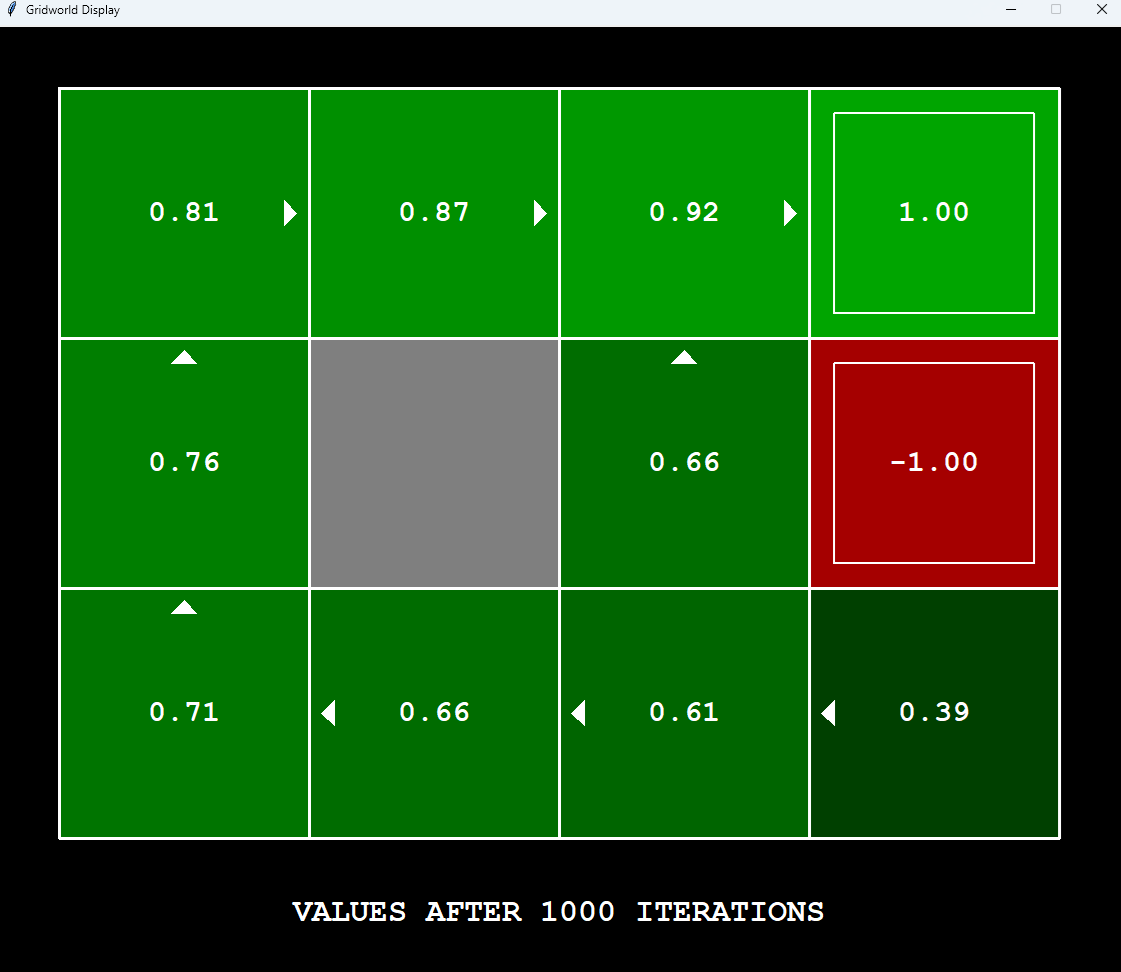
\includegraphics[width=0.80\textwidth]{figures/gridworld_values.png}
	\label{fig:gridworld_values}
\end{figure}

\end{frame}


\begin{frame}{Toy Maze Example (No Learning, Noise 20\%)}
\begin{figure}
	\centering
		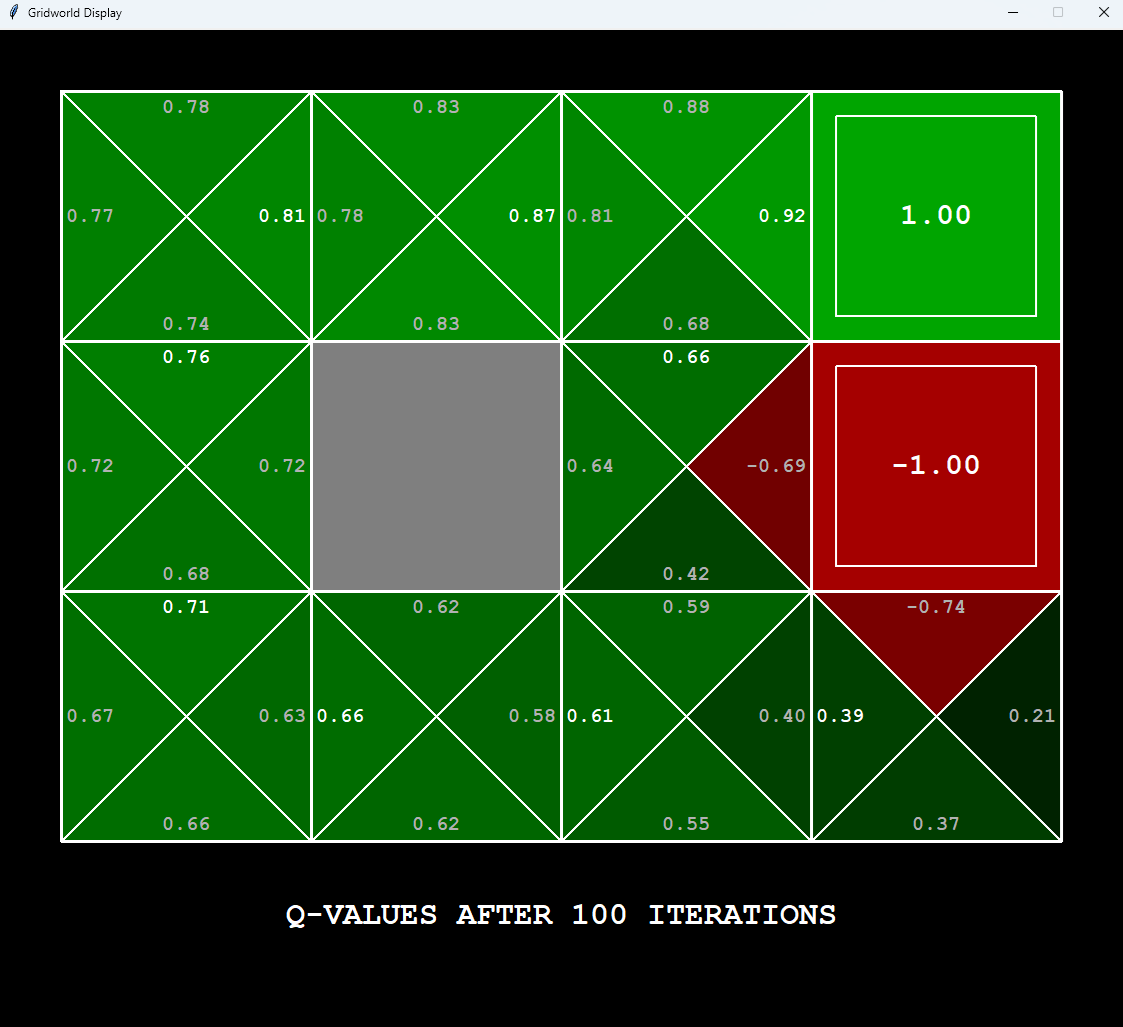
\includegraphics[width=0.80\textwidth]{figures/gridworld_qvalues.png}
	\label{fig:gridworld_values}
\end{figure}

\end{frame}

\begin{frame}{Toy Maze Example ($\varepsilon=0.9$, Noise 20\%)}
\begin{figure}
	\centering
		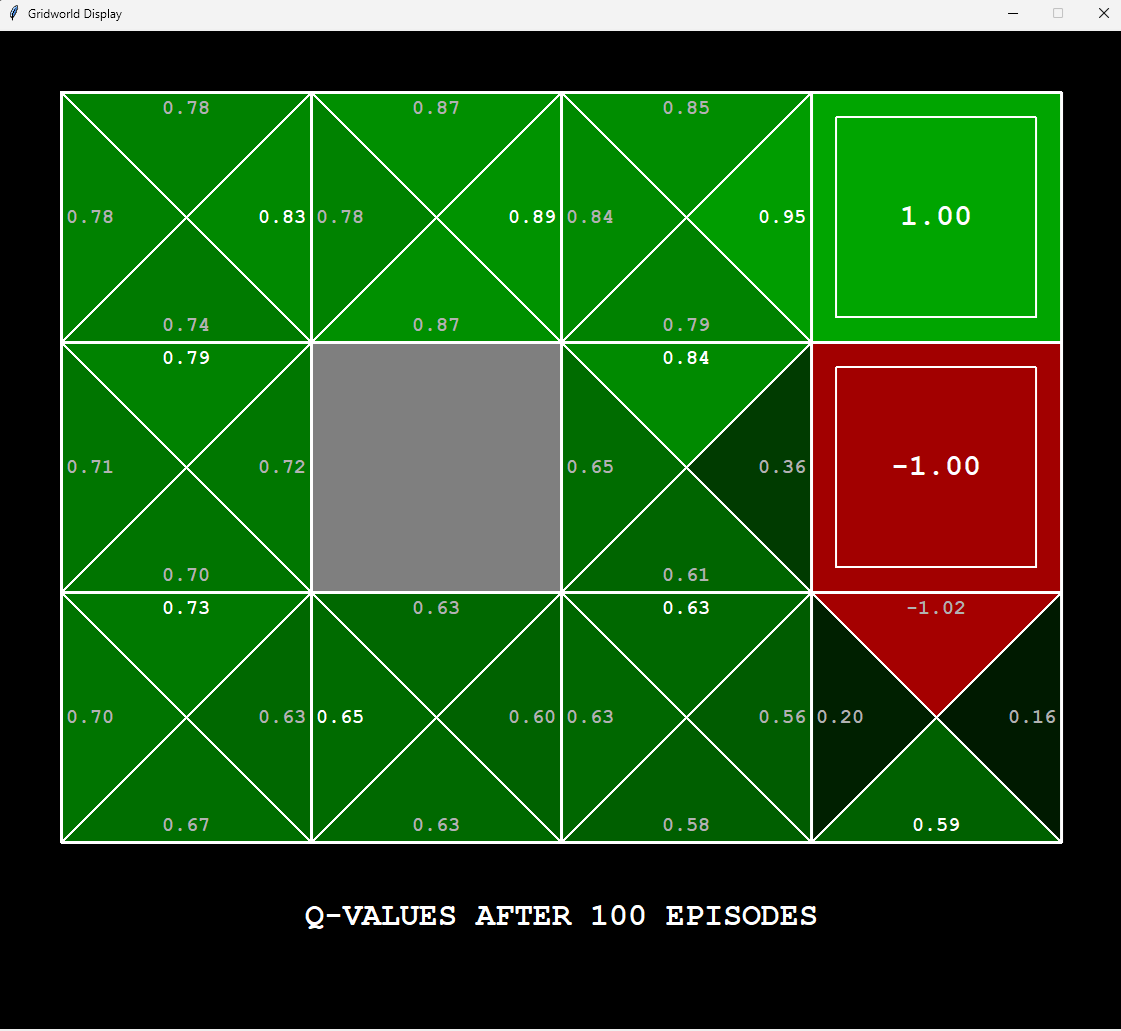
\includegraphics[width=0.80\textwidth]{figures/gridworld_qvalues_epsilon90.png}
	\label{fig:gridworld_values}
\end{figure}
Average reward: -1.14
\end{frame}

\begin{frame}{Toy Maze Example ($\varepsilon=0.1$, Noise 20\%)}
\begin{figure}
	\centering
		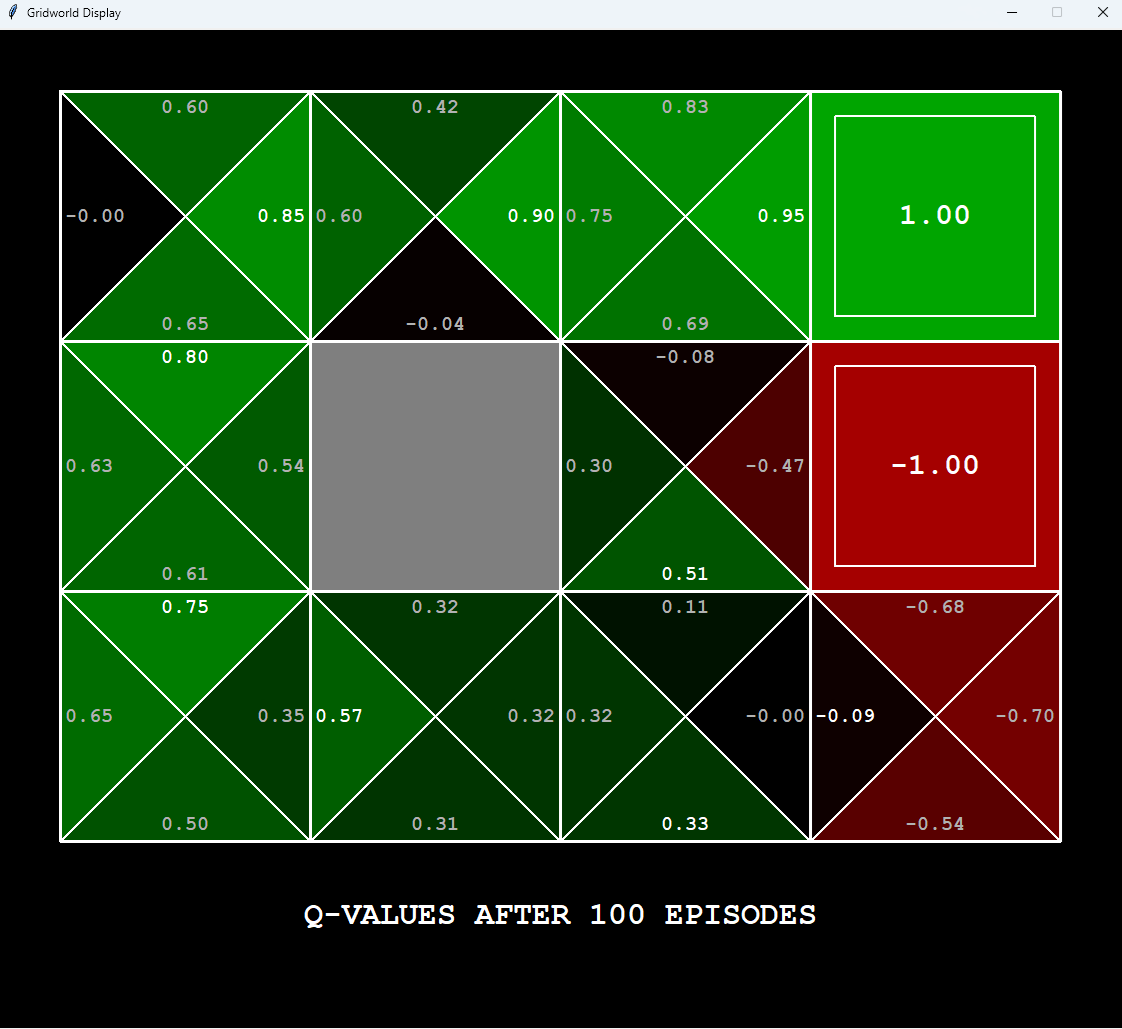
\includegraphics[width=0.80\textwidth]{figures/gridworld_qvalues_epsilon10.png}
	\label{fig:gridworld_values}
\end{figure}
Average reward: 0.0036
\end{frame}


\begin{frame}[t,allowframebreaks
]\nocite{*}
\frametitle{References}
\footnotesize
\bibliography{bib}
\end{frame}
\section{Takeaways}
{
\setbeamercolor{background canvas}{bg=BrewerBlue}
\begin{frame}
\centering
\Huge
\textcolor{white}{Takeaways}
\thispagestyle{empty}
\end{frame}
}

\begin{frame}{Learn Value of Taking Actions in Specific States}
\begin{itemize}
    \item Q-Learning learns optimal actions without knowing the model
    \item Balancing exploration and exploitation is crucial
    \item $\epsilon$-greedy and Boltzmann are common exploration methods
    \item Sufficient exploration guarantees convergence
\end{itemize}
\end{frame}


\end{document}
